 
\chapter{Branch Prediction}\label{chapter:bpd}

This chapter discusses how BOOM predicts branches and then resolves these predictions.

BOOM uses two levels of branch prediction- a single-cycle ``next-line predictor" (NLP) and a slower but more complex ``backing predictor" (BPD).\footnote{Unfortunately, the terminology in the literature gets a bit muddled here in what to call different types and levels of branch predictor. I have seen ``micro-BTB" versus ``BTB", ``NLP" versus ``BHT", and ``cache-line predictor" versus ``overriding predictor". 
Although the Rocket code calls its own predictor the ``BTB", I have chosen to refer to it in documentation as the ``next-line predictor", to denote that it is a combinational predictor that provides single-cycle predictions for fetching ``the next line", and the Rocket BTB encompasses far more complexity than just a ``branch target buffer" structure.  Likewise, I have chosen the name ``backing predictor" as I believe it is the most accurate name, while simultaneously avoiding being overly descriptive of the internal design (is it a simple BHT? Is it tagged? Does it override the NLP?).
{\color{red} But in short, I am open to better names!}}



\begin{figure}[ht]
	\centering
	\centerline{\includegraphics[scale =1] {figures/frontend}}
	\caption{ \small The Fetch Unit.}
	\label{fig:fetch}
\end{figure}


\section{The Rocket Next-line Predictor (NLP)}

BOOM instantiates the Rocket core's Front-End, which fetches instructions and predicts every cycle where to fetch the next instructions. If a misprediction is detected in BOOM's backend, or BOOM's own backing predictor wants to redirect the pipeline in a different direction, a request is sent to the Front-End and it begins fetching along a new instruction path. 

The next-line predictor (NLP) takes in the current PC being used to fetch instructions (the {\em Fetch PC}) and predicts combinationally where the next instructions should be fetched for the next cycle. If predicted correctly, there are no pipeline bubbles. 

The next-line predictor is an amalgamation of a fully-associative branch target buffer (BTB), a {\em gshare} branch history table (BHT), and a return address stack (RAS) which work together to make a fast, but reasonably accurate prediction.

\subsection{NLP Predictions}

The {\em Fetch PC} first performs a tag match to find a uniquely matching BTB entry.  
If a hit occurs, the BTB entry will make a prediction in concert with the BHT and RAS as to whether there is a branch, jump, or return found in the {\em fetch packet} and which instruction in the {\em fetch packet} is to blame.  
The BTB entry also contains a predicted PC target, which is used as the {\em Fetch PC} on the next cycle.


\begin{figure}[ht]
	\centering
	\centerline{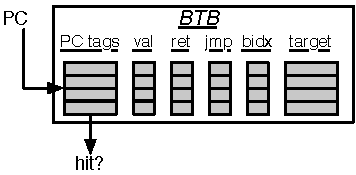
\includegraphics[scale =1] {figures/btb}}
	\caption{ \small The Next-line Predictor (NLP) Unit. The Fetch PC scans the BTB's ``PC tags'' for a match.  If a match is found (and the entry is valid), the BHT and RAS are consulted for the final verdict.  If the entry is a ``ret'' ({\em return} instruction), then the target comes from the RAS.  If the entry is a unconditional ``jmp'' ({\em jump} instruction), then the BHT is not consulted. The ``bidx'', or branch index, marks which instruction in a superscalar fetch packet is the cause of the control flow prediction. This is necessary to mask off the other instructions in the fetch packet that come over the taken branch.}
	\label{fig:btb}
\end{figure}




The hysteresis bits (governed by a {\em gshare} predictor) are only used on a BTB entry {\em hit} and if the predicting instruction is a branch.

If the BTB entry contains a {\em return} instruction, the RAS stack is used to provide the predicted return PC as the next {\em Fetch PC}. The actual RAS management (of when to {\tt {pop}} or {\tt {push}} the stack) is governed externally. 

For area-efficiency, the high-order bits of the PC tags and PC targets are stored in a compressed file.


\subsection{NLP Updates}

Each branch passed down the pipeline remembers not only its own PC, but also its {\em Fetch PC} (the PC of the head instruction of its {\em fetch packet}).\footnote{In reality, only the very lowest bits must be saved, as the higher-order bits will be the same.}  



\subsubsection{BTB Updates}

The BTB is updated {\bf only} when the Fetch Unit is redirected to {\bf take} a branch or jump by either the Branch Unit (in the {\em Execute} stage) or the Backing Predictor (in the {\em Branch Predict} stage).\footnote{Rocket's BTB relies on a little cleverness - when redirecting the PC on a misprediction, this new {\em Fetch PC } is the same as the {\em Update PC} that needs to be written into a new BTB entry's {\em Target PC} field. This ``coincidence" allows the PC compression table to use a single search port - it is simultaneously reading the table for the next prediction while also seeing if the new {\em Update PC} already has the proper high-order bits allocated for it.}

If there is no BTB entry corresponding to the taken branch or jump, an new entry is allocated for it.

\subsubsection{BHT Updates}

The BHT is composed of two parts that require updates - a {\em global history (ghistory)} register and a table of {\em history counters}. 

The \ghistory\ register tracks the outcomes of the last $N$ branches that have been fetched. It must be updated:

\begin{itemize}
\item in the {\em Branch Predict} stage - once we have decoded the instruction {\em fetch bundle}, know if any branches are present, and which direction the branch predictors have chosen to direct the Fetch Unit.
\item in the {\em Execute} stage - if and only if a {\em misprediction} occurs, the \ghistory\ register must be reset with the correct outcome of the branch history.
\end{itemize}

The {\em history counter} table is updated when the \ghistory\ register is updated.  Because the counters are read out and passed down the pipeline with the branch instruction, there is not a problem with having updated the counters incorrectly in the earlier {\em Branch Predict} stage. If a misprediction occurs, the counters will be reset and incremented to the proper value.

Notice that by updating the history counters in the {\em Branch Predict} stage, the updates are being performed in-order!  However, it is possible for a branch to update the {\em history counters} before later being found to have been misspeculated under a previous branch. We suspect that this is a fairly benign scenario.\footnote{Likewise, the BHT does not keep track of a {\em commit copy} of the \ghistory\ register.  This means that any sort of exceptions or pipeline replays will leave the \ghistory\ register in an incoherent state.  However, experiments showed that this had no noticeable effect on performance on real benchmarks.  This is probably because the BHT's \ghistory\ register is fairly small and can quickly re-learn the history in only a few cycles.}


\subsubsection{RAS Updates}

The RAS is updated during the {\em Branch Predict} stage once the instructions in the {\em fetch packet} have been decoded. If the taken instruction is a call\footnote{While RISC-V does not have a dedicated {\tt {CALL}} instruction, it can be inferred by checking for a {\tt {JAL}} or {\tt {JALR}} instruction with a writeback destination to {\tt {x1}} (aka, the {\tt {return address register}}).}, the {\em Return Address} is {\tt {pushed}} onto the RAS. If the taken instruction is a {\tt {RETURN}}, then the RAS is {\tt {popped}}.

\subsubsection{Superscalar Predictions}


When the NLP makes a prediction, it is actually using the BTB to tag match against the predicted branch's {\em Fetch PC}, and not the PC of the branch itself.  
The NLP must predict across the entire {\em fetch packet} which of the many possible branches will be the dominating branch that redirects the PC.
For this reason, we use a given branch's {\em Fetch PC} rather than its own PC in the BTB tag match.\footnote{Each BTB entry corresponds to a single {\em Fetch PC}, but it is helping to predict across an entire {\em fetch packet}. However, the BTB entry can only store meta-data and target-data on a single control-flow instruction.  While there are certainly pathological cases that can harm performance with this design, the assumption is that there is a correlation between which branch in a {\em fetch packet} is the dominating branch relative to the {\em Fetch PC}, and - at least for narrow fetch designs - evaluations of this design has shown it is very complexity-friendly with no noticeable loss in performance. Some other designs instead choose to provide a whole bank of BTBs for each possible instruction in the {\em fetch packet}.} 


\section{The Backing Predictor (BPD)}


\begin{figure}[htp]
	\centering
	\centerline{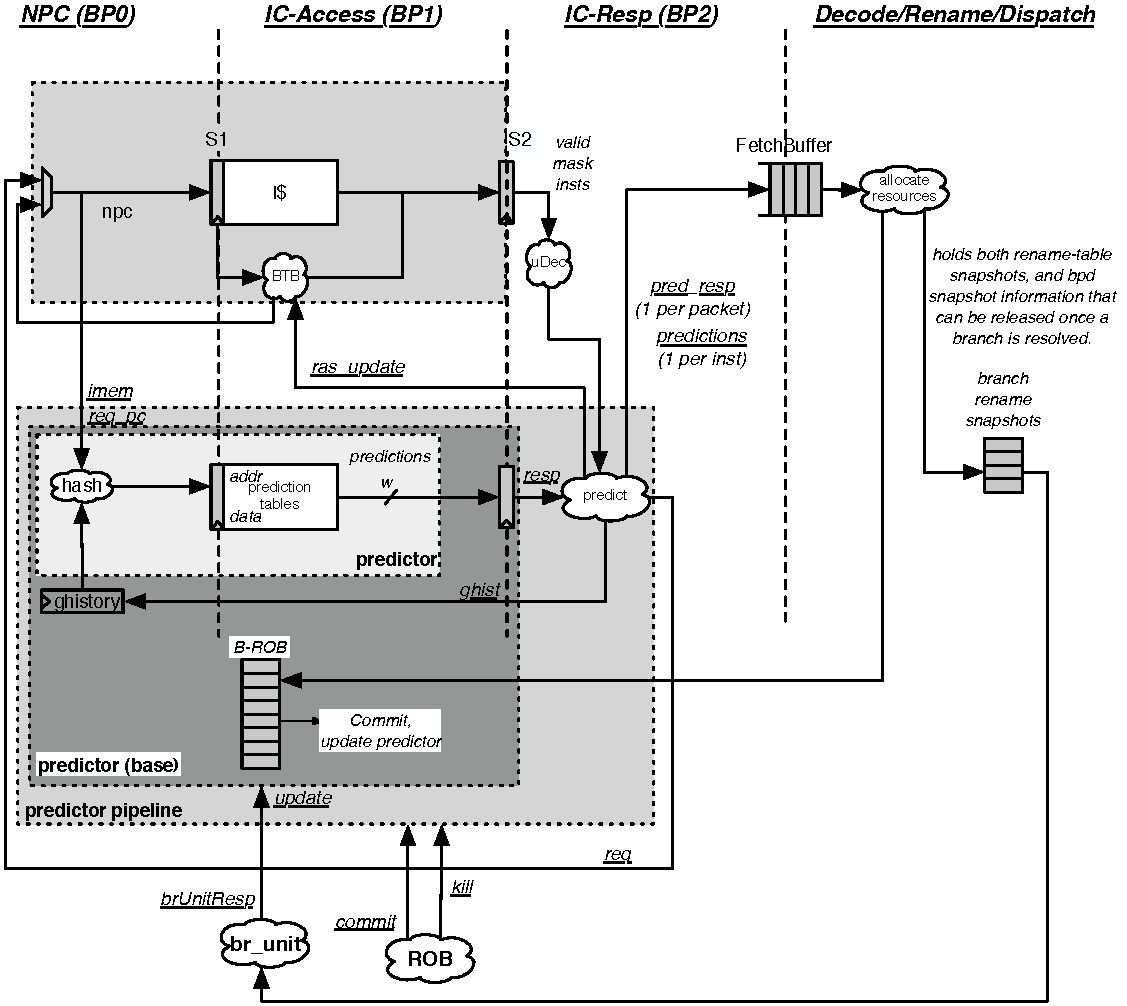
\includegraphics[scale =0.9] {figures/bpd}}
	\caption{ \small The Backing Branch Predictor (BPD) Unit. The front-end sends the ``next PC'' (npc) to the BPD ({\em BP0} stage).  A hash of the {\em npc} and the {\em global history} is used to index the predictor tables.  The predictor tables (ideally stored in SRAM) are accessed in parallel with the instruction cache ({\em BP1} stage). The BPD then returns a prediction for each instruction in the {\em fetch packet}. The instructions returning from the instruction cache are quickly decoded; any branches that are predicted as {\em taken} will redirect the front-end from the {\em BP2} stage.  Prediction snapshots and metadata are stored in the {\em branch rename snapshots} (for fixing the predictor after mispredictions) and the {\em Branch Re-order Buffer} (for updating the predictor in the {\em Commit} stage).}
	\label{fig:bpd}
\end{figure}

When the next-line predictor (NLP) is predicting well, the processor's backend is provided an unbroken stream of instructions to execute. The NLP is able to provide fast, single-cycle predictions by being expensive (in terms of both area and power), very small (only a few dozen branches can be remembered), and very simple (the {\em gshare} hysterisis bits are not able to learn very complicated or long history patterns).

To capture more branches and more complicated branching behaviors, BOOM provides support for a ``Backing Predictor", or BPD (see Figure \ref{fig:bpd}).

The BPD's goal is to provide very high accuracy in a (hopefully) dense area.  To make this possible, the BPD will not make a prediction until the {\em fetch packet} has been decoded and the branch targets computed directly from the instructions themselves.  This saves on needing to store the {\em PC tags} and {\em branch targets} within the BPD.\footnote{It's the {\em PC tag} storage and {\em branch target} storage that makes the BTB within the NLP so expensive.}

The BPD is accessed in parallel with the instruction cache access (See Fig. \ref{fig:fetch}).  This allows the BPD to be stored in sequential memory (i.e., SRAM instead of flip-flops). With some clever architecting, the BPD can be stored in single-ported SRAM to achieve the density desired~\cite{seznec2002design}.

\subsection{Making Predictions}

When making a prediction, the backing predictor must provide the following:

\begin{itemize}
\item is a prediction being made?
\item a bit-vector of taken/not-taken predictions
\end{itemize}

As per the first bullet-point, the BPD may decide to not make a prediction. This may be because the predictor uses tags to inform whether its prediction is valid or there may be a structural hazard that prevented a prediction from being made.

The BPD provides a bit-vector of taken/not-taken predictions, the size of the bit-vector matching the {\em fetch width} of the pipeline (one bit for each instruction in the {\em fetch packet}). The {\em Branch Prediction} stage will decode the instructions in the {\em fetch packet}, compute the branch targets, and decide in conjunction with the BPD's prediction bit-vector if a front-end redirect should be made. 

\subsubsection{Jump and Jump-Register Instructions}

The BPD makes predictions only on the direction (taken versus not-taken) of conditional branches.  Non-conditional ``jumps" (\jal) and ``jump-register" (\jalr) instructions are handled separately from the BPD.\footnote{\jal\ instructions jump to a $PC+Immediate$ location, whereas \jalr\ instructions jump to a $PC+Register[rs1]+Immediate$ location.}

The NLP learns any ``taken" instruction's {\em PC} and {\em target PC} - thus, the NLP is able to predict jumps and jump-register instructions.

If the NLP does not make a prediction on a \jal\ instruction, the pipeline will redirect the Fetch Unit in the {\em Fetch2 Stage} (see Fig. \ref{fig:fetch}).\footnote{Redirecting the Fetch Unit in the {\em Fetch2 Stage} for \jal\ instructions is trivial, as the instruction can be decoded and its target can be known.}

Jump-register instructions that were not predicted by the NLP will be sent down the pipeline with no prediction made.  As \jalr\ instructions require reading the register file to deduce the jump target, there's nothing that can be done if the NLP does not make a prediction.


\subsection{Updating the Backing Predictor}

Generally speaking, the BPD is updated during the {\em Commit} stage. This prevents the BPD from being polluted by wrong-path information.\footnote{In the data-cache, it can be useful to fetch data from the wrong path- it is possible that future code executions may want to access the data. Worst case, the cache's effective capacity is reduced. But it can be quite dangerous to add wrong-path information to the BPD - it truly represents a code-path that is never exercised, so the information will {\em never} be useful in later code executions. Worst, aliasing is a problem in branch predictors (at most partial tag checks are used) and wrong-path information can create deconstructive aliasing problems that worsens prediction accuracy.  Finally, bypassing of the inflight prediction information can occur, eliminating any penalty of not updating the predictor until the {\em Commit} stage.}  
However, as the BPD makes use of global history, this history must be reset whenever the Fetch Unit is redirected. Thus, the BPD must also be (partially) updated during {\em Execute} when a misprediction occurs to reset any speculative updates that had occurred during the {\em Fetch} stages.

When making a prediction, the BPD passes to the pipeline a ``response info packet".  This ``info packet" is stored in a ``branch re-order buffer" (BROB) until commit time.\footnote{These {\em info packets} are not stored in the ROB for two reasons - first, they correspond to {\em fetch packets}, not instructions.  Second, they are very expensive and so it is reasonable to size the BROB to be smaller than the ROB.}  Once all of the instructions corresponding to the ``info packet" is committed, the ``info packet" is set to the BPD (along with the eventual outcome of the branches) and the BPD is updated. Section \ref{sec:brob} covers the BROB, which handles the snapshot information needed for update the predictor during {\em Commit}. Section \ref{sec:bpd-rename} covers the BPD Rename Snapshots, which handles the snapshot information needed to update the predictor during a misspeculation in the {\em Execute} stage.

\subsection{Managing the Global History Register}\label{sec:ghistory}

The {\em global history register} is an important piece of a branch predictor. It contains the outcomes of the previous $N$ branches (where $N$ is the size of the global history register).\footnote{Actually, the direction of all conditional branches within a {\em fetch packet} are compressed (via an OR-reduction) into a single bit, but for this section, it is easier to describe the history register in slightly inaccurate terms.}

When fetching branch $i$, it is important that the direction of the previous $i-N$ branches is available so an accurate prediction can be made.  Waiting till the {\em Commit} stage to update the global history register would be too late (dozens of branches would be inflight and not reflected!). Therefore, the global history register must be updated {\em speculatively}, once the branch is fetched and predicted in the {\em BP2} stage.

If a misprediction occurs, the global history register must be reset and updated to reflect the actual history.  This means that each branch (more accurately, each {\em fetch packet}) must snapshot the global history register in case of a misprediction.\footnote{Notice that there is a delay between beginning to make a prediction in the {\em BP0} stage (when the global history is read) and redirecting the front-end in the {\em BP2} stage (when the global history is updated).  This results in a ``shadow'' in which a branch beginning to make a prediction in {\em BP0} will not see the branches (or their outcomes) that came a cycle (or two) earlier in the program (that are currently in {\em BP1} or {\em BP2} stages).  It is vitally important though that these ``shadow branches'' be reflected in the global history snapshot.}

There is one final wrinkle - exceptional pipeline behavior.  While each branch contains a snapshot of the global history register, any instruction can potential throw an exception that will cause a front-end redirect. Such an event will cause the global history register to become corrupted. For exceptions, this may seem acceptable - exceptions should be rare and the trap handlers will cause a pollution of the global history register anyways (from the point of view of the user code).  However, some exceptional events include ``pipeline replays" - events where an instruction causes a pipeline flush and the instruction is refetched and re-executed.\footnote{An example of a pipeline replay is a {\em memory ordering failure} in which a load executed before an older store it depends on and got the wrong data. The only recovery requires flushing the entire pipeline and re-executing the load.}  For this reason, a {\em commit copy} of the global history register is also maintained by the BPD and reset on any sort of pipeline flush event.

\subsection{The Branch Reorder Buffer (BROB)}\label{sec:brob}

The Reorder Buffer (see Chapter \ref{chapter:rob}) maintains a record of all inflight instructions. Likewise, the Branch Reorder Buffer (BROB) maintains a record of all inflight branch predictions.  These two structure are decoupled as BROB entries are {\em incredibly} expensive and not all ROB entries will contain a branch instruction. As only roughly one in every six instructions is a branch, the BROB can be made to have fewer entries than the ROB to leverage additional savings.

Each BROB entry corresponds to a single superscalar branch prediction. Said another way, there is a 1:1 correspondence between a single fetch cycle's prediction and a BROB entry.  
For each prediction made, the branch predictor packs up data that it will need later to perform an update. For example, a branch predictor will want to remember what {\em index} a prediction came from so it can update the counters at that index later. This data is stored in the BROB. 

When the last instruction in a fetch group is committed, the BROB entry is deallocated and returned to the branch predictor.  Using the data stored in the BROB entry, the branch predictor can perform any desired updates to its prediction state. 

There are a number of reasons to update the branch predictor after {\em Commit}. It is crucial that the predictor only learns {\em correct} information. In a data cache, memory fetched from a wrong path execution may eventually become useful when later executions go to a different path.  But for a branch predictor, wrong path updates encode information that is pure pollution -- it takes up useful entries by storing information that is not useful and will never be useful.  Even if later iterations do take a different path, the history that got it there will be different. And finally, while caches are fully tagged, branch predictors use partial tags (if any) and thus suffer from deconstructive aliasing.

Of course, the latency between {\em Fetch} and {\em Commit} is inconvenient and can cause extra branch mispredictions to occur if multiple loop iterations are inflight. However, the BROB could be used to bypass branch predictions to mitigate this issue. Currently, this bypass behavior is not supported in BOOM.

The BROB is broken up into two parts: the prediction {\em data} and the branch execution {\em metadata}.  The metadata tracks which instructions within the fetch packet where branches, which direction they took, and which branches were mispredicted (this requires random access). The prediction data is written once into the BROB upon instruction {\em Dispatch} and read out (and deallocated) during {\em Commit}.


\subsection{Rename Snapshot State}\label{sec:bpd-rename}

The BROB holds branch predictor data that will be needed to update the branch predictor during {\em Commit} (for both correct and incorrect predictions).  However, there is additional state needed for when the branch predictor makes an incorrect prediction {\em and must be updated immediately}.  For example, if a misprediction occurs, the speculatively-updated global history must be reset to the correct value before the processor can begin fetching (and predicting) again. 

This state can be very expensive but it can be deallocated once the branch is resolved in the {\em Execute} stage. Therefore, the state is stored in parallel with the {\em Rename Snapshots}.  During {\em Decode} and {\em Rename}, a branch tag is allocated to each branch and a snapshot of the rename tables are made to facilitate single-cycle rollback if a misprediction occurs.  Like the branch tag and rename maptable snapshots, the corresponding branch predictor ``rename'' snapshot can be deallocated once the branch is resolved by the Branch Unit in {\em Execute}.



\subsection{The Abstract Branch Predictor Class}

To facilitate exploring different global history-based BPD designs, an abstract ``BrPredictor" class is provided.  It provides a standard interface into the BPD, the control logic for managing the global history register, and contains the {\em branch reorder buffer (BROB)} (which handles the inflight branch prediction checkpoints). This abstract class can be found in Figure \ref{fig:bpd} labeled ``predictor (base)''.

\subsubsection{Global History}

As discussed in Section \ref{sec:ghistory}, global history is a vital piece of any branch predictor.  As such, it is handled by the abstract BranchPredictor class.  Any branch predictor extending the abstract BranchPredictor class gets access to global history without having to handle  snapshotting, updating, and bypassing.

\subsubsection{Very Long Global History (VLHR)}\label{sec:vlhr}

Some branch predictors (see Section \ref{sec:tage}) require access to incredibly long histories -- over a thousand bits.  Global history is speculatively updated after each prediction and must be snapshotted and reset if a misprediction was made. Snapshotting a thousand bits is untenable.  Instead, VLHR is implemented as a circular buffer with a speculative head pointer and a commit head pointer.  As a prediction is made, the prediction is written down at $VLHR[spec\_head]$ and the speculative head pointer is incremented and snapshotted. When a branch mispredicts, the head pointer is reset to $snapshot+1$ and the correct direction is written to $VLHR[snapshot]$.  In this manner, each snapshot is on the order of 10 bits, not 1000 bits.


\subsubsection{Operating System-aware Global Histories}

Although the data on its benefits are preliminary, BOOM does support OS-aware global histories.  The normal global history tracks all instructions from all privilege levels. A second {\em user-only global history} tracks only user-level instructions. 

\subsection{The Two-bit Counter Tables}

The basic building block of most branch predictors is the ``Two-bit Counter Table'' (2BC).  As a particular branch is repeatedly taken, the counter saturates upwards to the max value 3 ({\em 0b11}) or {\em strongly taken}.  Likewise, repeatedly not-taken branches saturate towards zero ({\em 0b00}).  The high-order bit specifies the {\em prediction} and the low-order bit specifies the {\em hysteresis} (how ``strong'' the prediction is).


\begin{figure}[ht]
	\centering
	\centerline{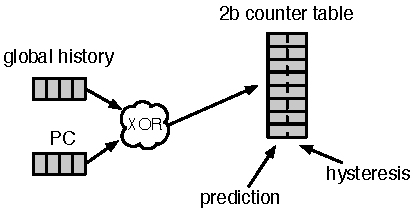
\includegraphics[scale =1.4] {figures/2bc-prediction}}
	\caption{ \small A {\em gshare} predictor uses the global history hashed with the PC to index into a table of 2-bit counters.  The high-order bit makes the prediction.}
	\label{fig:2bc-prediction}
\end{figure}


These two-bit counters are aggregated into a table. Ideally, a good branch predictor knows which counter to index to make the best prediction. However, to fit these two-bit counters into dense SRAM, a change is made to the 2bc finite state machine -- mispredictions made in the {\em weakly not-taken} state move the 2bc into the {\em strongly taken} state (and vice versa for {\em weakly taken} being mispredicted). The FSM behavior is shown in Figure \ref{fig:2bc-fsm}.

\begin{figure}[ht]
	\centering
	\centerline{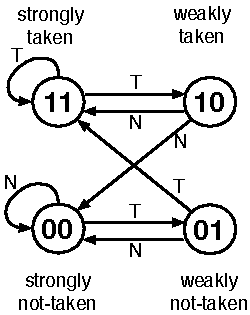
\includegraphics[scale =1] {figures/2bc-fsm}}
	\caption{ \small Two-bit counter state machine.}
	\label{fig:2bc-fsm}
\end{figure}

Although it's no longer strictly a ``counter", this change allows us to separate out the read and write requirements on the {\em prediction} and {\em hystersis} bits and place them in separate sequential memory tables. In hardware, the 2bc table can be implemented as follows:

\begin{quote}
The P-bit:
\begin{itemize}
\item {\bf read} - every cycle to make a prediction
\item {\bf write} - only when a misprediction occurred (the value of the h-bit).
\end{itemize}

The H-bit:

\begin{itemize}
\item {\bf read} - only when a misprediction occurred.
\item {\bf write} - when a branch is resolved (write the direction the branch took).
\end{itemize}
\end{quote}

By breaking the high-order p-bit and the low-order h-bit apart, we can place each in 1~read/1~write SRAM. A few more assumptions can help us do even better. Mispredictions are rare and branch resolutions are not necessarily occurring on every cycle. Also, writes can be delayed or even dropped altogether. Therefore, the {\em h-table} can be implemented using a single 1rw-ported SRAM by queueing writes up and draining them when a read is not being performed. Likewise, the {\em p-table} can be implemented in 1rw-ported SRAM by banking it -- buffer writes and drain when there is not a read conflict.


A final note: SRAMs are not happy with a ``tall and skinny'' aspect ratio that the 2bc tables require. However, the solution is simple -- tall and skinny can be trivially transformed into a rectangular memory structure.  The high-order bits of the index can correspond to the SRAM row and the low-order bits can be used to mux out the specific bits from within the row. 

\subsection{The GShare Predictor}

{\em Gshare} is a simple but very effective branch predictor. Predictions are made by hashing the instruction address and the global history (typically a simple XOR) and then indexing into a table of two-bit counters.  Figure \ref{fig:2bc-prediction} shows the logical architecture and Figure \ref{fig:gshare} shows the physical implementation and structure of the {\em gshare} predictor. Note that the prediction begins in the BP0 stage when the requesting address is sent to the predictor but that the prediction is made later in the BP2 stage once the instructions have returned from the instruction cache and the prediction state has been read out of the {\em gshare}'s p-table.


\begin{figure}[ht]
	\centering
	\centerline{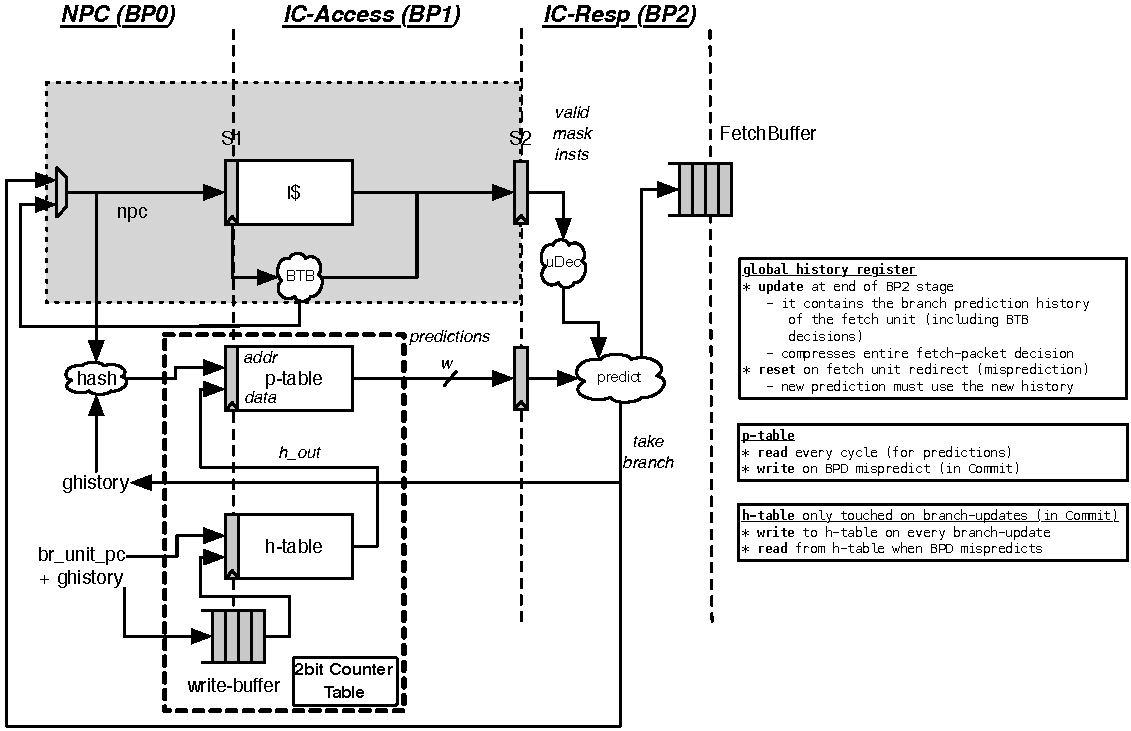
\includegraphics[scale =0.95] {figures/gshare}}
	\caption{ \small The GShare predictor pipeline.}
	\label{fig:gshare}
\end{figure}

\subsection{The TAGE Predictor}\label{sec:tage}

BOOM also implements the TAGE conditional branch predictor. TAGE is a highly-parameterizable, state-of-the-art global history predictor~\cite{seznec2006case, seznec2011new}.  The design is able to maintain a high degree of accuracy while scaling from very small predictor sizes to very large predictor sizes. It is fast to learn short histories while also able to learn very, very long histories (over a thousand branches of history).  


\begin{figure}[ht]
	\centering
	\centerline{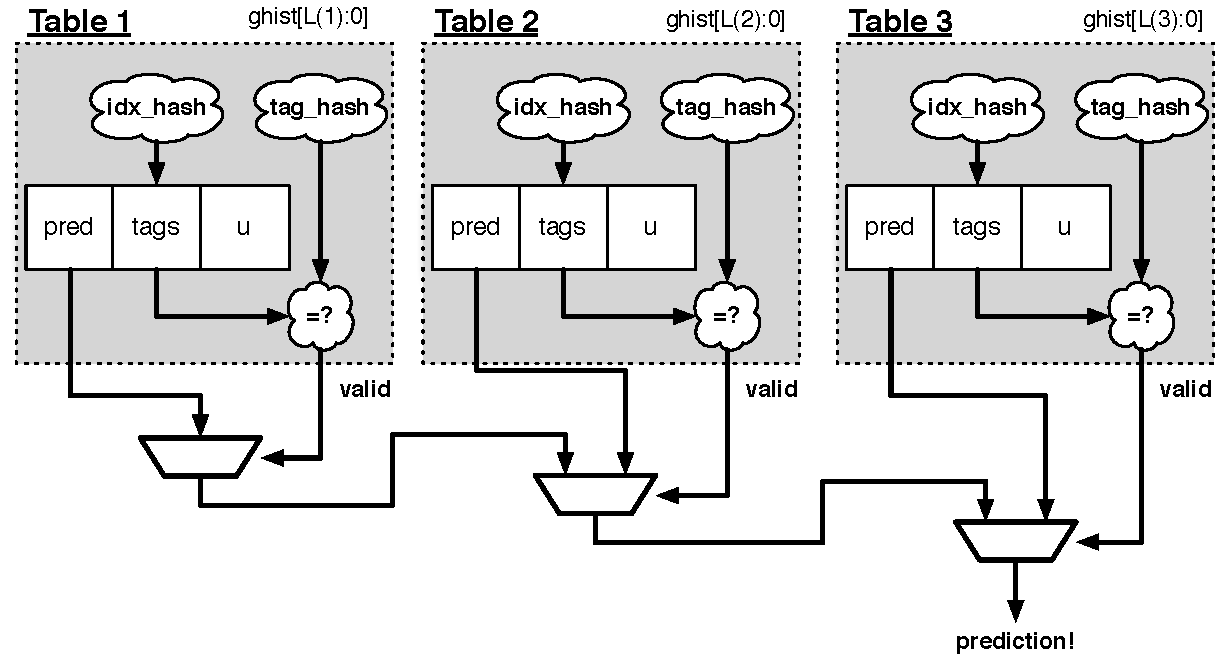
\includegraphics[scale =0.80] {figures/tage}}
	\caption{ \small The TAGE predictor. The requesting address (PC) and the global history are fed into each table's index hash and tag hash. Each table provides its own prediction (or no prediction) and the table with the longest history wins.}
	\label{fig:tage}
\end{figure}


TAGE (TAgged GEometric) is implemented as a collection of predictor tables. Each table entry contains a {\em prediction counter}, a {\em usefulness counter}, and a {\em tag}. The {\em prediction counter} provides the prediction (and maintains some hysteresis as to how strongly biased the prediction is towards taken or not-taken). The {\em usefulness counter} tracks how useful the particular entry has been in the past for providing correct predictions.  The {\em tag} allows the table to only make a prediction if there is a tag match for the particular requesting instruction address and global history.

Each table has a different (and geometrically increasing) amount of history associated with it.  Each table's history is used to hash with the requesting instruction address to produce an index hash and a tag hash.  Each table will make its own prediction (or no prediction, if there is no tag match).  The table with the longest history making a prediction wins. 

On a misprediction, TAGE attempts to allocate a new entry. It will only overwrite an entry that is ``not useful'' ($ubits == 0$). 

\subsubsection{TAGE Global History and the Circular Shift Registers (CSRs)\protect\footnote{No relation to the Control/Status Registers.}}

Each TAGE table has associated with it its own global history (and each table has geometrically more history than the last table). As the histories become incredibly long (and thus too expensive to snapshot directly), TAGE uses the Very Long Global History Register (VLHR) as described in Section \ref{sec:vlhr}.  The histories contain many more bits of history that can be used to index a TAGE table; therefore, the history must be ``folded'' to fit. A table with 1024 entries uses 10 bits to index the table. Therefore, if the table uses 20 bits of global history, the top 10 bits of history are XOR'ed against the bottom 10 bits of history. 

Instead of attempting to dynamically fold a very long history register every cycle, the VLHR can be stored in a circular shift register (CSR).  The history is stored already folded and only the new history bit and the oldest history bit need to be provided to perform an update. Code \ref{code:tage-csr} shows an example of how a CSR works. 

\begin{center}
\begin{minipage}{0.90\textwidth}
\begin{lstlisting}[caption={The circular shift register. When a new branch outcome is added, the register is shifted (and wrapped around). The new outcome is added and the oldest bit in the history is ``evicted''.}]
Example:   
  A 12 bit value (0b_0111_1001_1111) folded onto a 5 bit CSR becomes 
  (0b_0_0010), which can be found by:                                       
                                                                             
                                                                             
               /-- history[12] (evict bit)                                   
               |                                                             
 c[4], c[3], c[2], c[1], c[0]                                                
  |                        ^                                                 
  |                        |                                                 
  \_______________________/ \---history[0] (newly taken bit)                 
                                                                             
                                                                             
(c[4] ^ h[ 0] generates the new c[0]).                                        
(c[1] ^ h[12] generates the new c[2]).       
\end{lstlisting}\label{code:tage-csr}
\end{minipage}
\end{center}                                 

Each table must maintain {\em three} CSRs.  The first CSR is used for computing the index hash and has a size $n=log(num\_table\_entries)$.  As a CSR contains the folded history, any periodic history pattern matching the length of the CSR will XOR to all zeroes (potentially quite common).  For this reason, there are two CSRs for computing the tag hash, one of width $n$ and the other of width $n-1$. 

For every prediction, all three CSRs (for every table) must be snapshotted and reset if a branch misprediction occurs. 
Another three {\em commit copies} of these CSRs must be maintained to handle pipeline flushes. 


\subsubsection{Usefulness counters (u-bits)}

The ``usefulness'' of an entry is stored in the {\em u-bit} counters.  Roughly speaking, if an entry provides a correct prediction, the u-bit counter is incremented. If an entry provides an incorrect prediction, the u-bit counter is decremented.  When a misprediction occurs, TAGE attempts to allocate a new entry.  To prevent overwriting a useful entry, it will only allocate an entry if the existing entry has a usefulness of zero.  However, if an entry allocation fails because all of the potential entries are useful, then all of the potential entries are decremented to potentially make room for an allocation in the future.

To prevent TAGE from filling up with only useful but rarely-used entries, TAGE must provide a scheme for ``degrading'' the u-bits over time.  A number of schemes are available.  One option is a timer that periodically degrades the u-bit counters.  Another option is to track the number of failed allocations (incrementing on a failed allocation and decremented on a successful allocation). Once the counter has saturated, all u-bits are degraded. 

\subsubsection{TAGE Snapshot State}

For every prediction, all three CSRs (for every table) must be snapshotted and reset if a branch misprediction occurs.  
TAGE must also remember the index of each table that was checked for a prediction (so the correct entry for each table can be updated later). 
Finally, TAGE must remember the tag computed for each table -- the tags will be needed later if a new entry is to be allocated.\footnote{There are ways to mitigate some of these costs, but this margin is too narrow to contain them.}
%\footnote{Although it is tempting to try and recompute the indices and tags to save on storage space, the problem with recomputing during {\em Commit} is that it would require having the {\em fetch PC} and the {\em fetch-time} values of the CSRs available to recreate the hashes.  As the CSRs are the most expensive part of the TAGE snapshots, they are deallocated after the branch is resolved in the {\em Execute} stage as they are only required for fixing a branch misprediction.}

\subsection{Other Predictors}

BOOM provides a number of other predictors that may provide useful.

\subsubsection{The Null Predictor}

The Null Predictor is used when no BPD predictor is desired. It will always predict ``not taken".

\subsubsection{The Random Predictor}

The Random Predictor uses an LFSR to randomize both ``was a prediction made?" and ``which direction each branch in the {\em fetch packet} should take?".  This is very useful for both torturing-testing BOOM and for providing a worse-case performance baseline for comparing branch predictors.

\section{Branch Prediction Configurations}

There are a number of parameters provided to govern the branch prediction in BOOM.

\subsection{GShare Configuration Options}

\subsubsection{Global History Length}

How long of a history should be tracked?  The length of the global history sets the size of the branch predictor. An $n$-bit history pairs with a $2^n$ entry two-bit counter table. 

\subsection{TAGE Configurations}

\subsubsection{Number of TAGE Tables}

How many TAGE tables should be used?

\subsubsection{TAGE Table Sizes}

What size should each TAGE table be?

\subsubsection{TAGE Table History Lengths}

How long should the global history be for each table? This should be a geometrically increasing value for each table.

\subsubsection{TAGE Table Tag Sizes}

What size should each tag be?

\subsubsection{TAGE Table U-bit Size}

How many bits should be used to describe the usefulness of an entry?

